\chapter{A quick introduction to EzQL}
\label{chap:ezql}

In this chapter we introduce EzQL, our proposal to attack the issues
outlined in the previous chapter. Its main features are:

\begin{itemize}
\item The language integrates both pulse and state-changes semantics,
  discussed in the previous chapter. Thus, \emph{EzQL does not lose
    any ability offered by current systems}, while it also adds new
  capabilities;
\item Includes a simple modeling approach, akin to object-orientation,
  where real-world entities can be modeled as objects with properties
  --- temperature, price or speed, for example ---, whose values
  depend on the values of events. For instance, this entity-model
  allows the creation of many Room entities each with their own
  temperature attribute which is automatically updated as new sensor
  readings arrive. Furthermore, these entities and the values of their
  properties define the state of the application and this state can be
  queried just like regular events;
\item The entity model supports \emph{associations} between entities,
  inspired by Ob\-ject-Relational Mapping (O/RM) tools for
  databases. Thus, it is possible to say, for instance, that a room
  has many products and, correspondingly, that a product belongs to
  one room. Again, these associations may change as new events arrive,
  i.e., a product may leave one room and enter another. Naturally,
  these relationships can also be queried --- one can ask, for
  example, what is the cheapest product inside room A. This type of
  queries can already be written in currently available systems, but
  we will see that they become much simpler in EzQL;
\item EzQL tries to give more power to the developer, allowing him to
  create user-defined aggregators and functions. It also supports
  higher-order functions, an important medium to create new
  abstractions;
\item It comes with a static type-system supporting type-inference and
  parametric polymorphism. This increases the expressiveness of the
  language without loosing the capability to check and guarantee that
  programs are type-safe.
\end{itemize}


\lstset{
  language=EzQL,
  columns=fullflexible,
  basicstyle=\tt,
  keywordstyle=[1]\bf,
  keywordstyle=[2]\it,
  tabsize=8,
  showtabs=true,
  tab=$\hspace{1pt}$
}

\section{Streams and windows}
\label{sec:streams-windows}

As we will see, EzQL is very different from the query languages
presented in the state of the art. However, at its core, it still has
streams of events and operations to query them.

Suppose you are given a stream called \verb=stocks= that receives
events from the financial market. These events contain three fields --
\verb=timestamp=, \verb=symbol= -- which is the company id --, and
\verb=price=. In EzQL you would start by declaring this stream with:

\begin{lstlisting}
  stocks = stream of { timestamp:int, symbol:string, price:float }
\end{lstlisting}

Now, the stream is ready to be used and you may query its data. For
example, to multiply the price of ACME events by two, you could write:

\begin{lstlisting}
  acmeStocks_x2 =
    from ev in stocks			# For each event ev in the stream
    where ev.symbol == "ACME"
    select { price_x2 = ev.price * 2 }
\end{lstlisting}

The syntax is inspired in SQL and that is only natural, as SQL handles
these simple queries very well. The only bit that deserves some
explanation is the segment between braces after \verb=select=. This
creates an event with one field -- \verb=price_x2= --, which we define
as twice the price held by the original event. The \verb=select=
operator implicitly adds a second field to the event -- the
\verb=timestamp= --, which is copied from the original event being
projected.

The result of this operation is a new stream --
\verb=acmeStocks_x2=. The next listing shows off a few more features
that EzQL shares with other languages, namely temporal windows and
aggregations:

\begin{lstlisting}
  avg_5min =
    let cheapStocks =
      from ev in stocks[5 min] 	 # For each event in the 5 min window
      where ev.price < 20
    cheapStocks.avg (:price)
\end{lstlisting}

This example computes the average price of all events received during
the last 5 minutes where the price is under \$20. The query has been
partitioned into two smaller sub-queries: the first --
\verb=cheapStocks= --, is a local variable declared using \verb=let=
that contains a stream with the filtered events, and the second is the
application of the \verb=avg()= method over \verb=cheapStocks=. To
understand this query, the reader should know that, in EzQL as in
other languages such as Python, indentation is significant. This
means that instead of using \verb=begin= and \verb=end= or \verb={=
  and \verb=}= to denote code blocks, we simply align related
statements using whitespace.

The resulting number is stored in \verb=avg_5min= and we may use it in
other queries. For example, to check if the average is smaller than 10
we could write:

\begin{lstlisting}
  isSmall = avg_5min < 10	# This is a query!
\end{lstlisting}

While it may seem uninteresting, this example illustrates one
important point that is essential to understand EzQL: \verb=isSmall=
is a continuously running query. Every time the average price changes,
the number stored in \verb=avg_5min= is updated, which then triggers
the re-computation of \verb=isSmall=. The engine works like a
spread-sheet application where a modification to one cell is
automatically propagated to other cells that depend on the first, and
so on.

\section{Continuous values}
\label{sec:continuous-values}

This example also shows the first major difference between EzQL and
other ESP languages: in EzQL, the result of an aggregator such as
\verb=avg()= is a continuous number and not a stream where events are
sporadically sent to every time the aggregated value changes. These
numbers are part of a large family of data types that we call
continuous values. The rationale behind the decision to introduce
continuous values instead of reusing streams is that, as we have seen
in chapter \ref{chap:simple-questions-complex-answers}, events are
ephemeral -- they come and, in the next instant, they are
gone. However, the maximum price over the last five minutes, for
example, will remain the same until a greater price arrives or the
current one expires. So, it makes sense to treat the maximum as a
continuous entity, whose value is always defined. However, in
traditional languages, if we need the current maximum at any time, we
must keep it inside a window with a single entry created specifically
for this purpose. We believe this represents an undesired level of
indirection that impacts the amount of code that needs to be written
and hides its meaning. It feels unnecessary to create a window when a
simple number would suffice. Thus, continuous values were born.

They are not restricted to numbers, though. For example,
\verb=isSmall= declared above is a continuous boolean that alternates
between \verb=true= and \verb=false=. All the other data types EzQL
supports (that we have yet to discuss) -- strings, records, tuples,
enumerations, closures, entities and dictionaries --, may be treated
as continuous entities.

Besides aggregators, the other primary operator that creates
continuous values is \verb=last()=. Conceptually, \verb=last()= works
by taking a stream that produces events and \emph{holding} each event
in sequence, until the arrival of the following event makes it
obsolete. Figure \ref{fig:last} illustrates this. This operator is
useful in many situations where the \emph{last} event defines the
\emph{current} state of the system. For example, an application that
manages financial data using the \verb=stocks= stream may consider the
current price of some company's stocks the same as the price that came
in the last event related to that company. According to this line of
reasoning, the current price of ACME could be found with:

\begin{figure}[t]
  \centering
  \subfloat[A regular stream.]{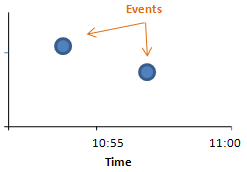
\includegraphics[width=0.4\textwidth]{last-a.png}}
  \subfloat[The same stream, after applying \tt last() \rm to hold its events.]{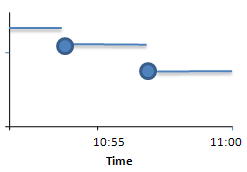
\includegraphics[width=0.4\textwidth]{last-b.png}}
  \caption{How \tt last() \rm works.}
  \label{fig:last}
\end{figure}


\begin{lstlisting}
  acmePrice =
    let acmeStocks =
      from ev in stocks
      where ev.symbol == "ACME"
    acmeStocks.last().price	 # Get the price from the last event
\end{lstlisting}

All continuous values may change as time passes or new events
arrive. As discussed, the system takes care of spreading these changes
automatically and transparently. However, in the same way that we can
create a window to analyze past events, we may also exploit the
temporal information contained in continuous values. As such, it is
possible to open windows and apply aggregators over regular integers,
booleans or other values. The following listing illustrates this:

\begin{lstlisting}
  maxAcme_1h = acmePrice[1 hour].max()
\end{lstlisting}

This results in the maximum price ACME's stocks attained over the
course of the last hour. Note that the 1 hour window is created over
\verb=acmePrice= -- that is, the continuous value that holds the
current price. You could have solved this by opening a regular event
window over the stream that contains only ACME's events:

\begin{lstlisting}
  maxAcme_1h_wrong =
    let acmeStocks =
      from ev in stocks
      where ev.symbol == "ACME"
    acmeStocks[1 hour].max(:price)
\end{lstlisting}

Surprisingly though, the results would differ. To see why, note that
this is just another instance of the pulse vs state-changes problem
discussed in section \ref{sec:acme-problem}: the price could have been
at its maximum 1 hour ago, but the notification for this value might
have happened a little earlier and thus, a regular sliding window
applied to a stream would not consider it when calculating the
maximum. A continuous value, on the other hand, retains its value
until a new event changes it. Thus, querying \verb=acmePrice= for its
maximum value over the last hour would consider all the values it had
during that time --- even if the corresponding event came earlier ---
and would give the correct result.

\begin{figure}[t]
  \centering
  \subfloat[maxAcme\_1h\_wrong]{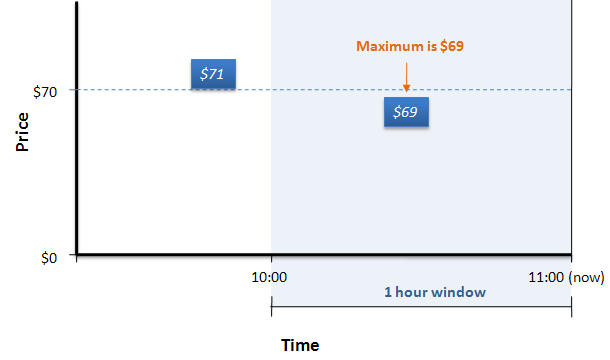
\includegraphics[width=0.5\textwidth]{maxAcme-wrong.png}}
  \subfloat[maxAcme\_1h]{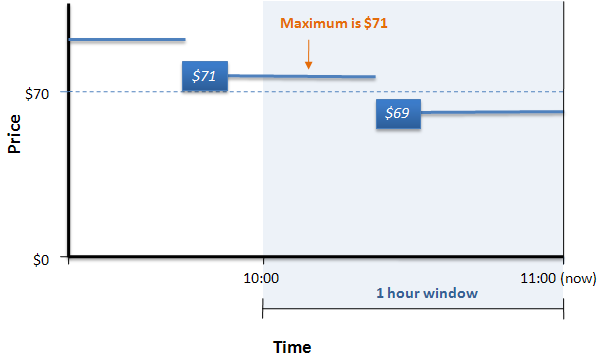
\includegraphics[width=0.5\textwidth]{maxAcme.png}}
  \caption{In the first case, the maximum is \$69 because only the
    second event lies inside the window. In the second, though, a
    continuous value is used to hold the higher price so that it still
    belongs to the window.}
  \label{fig:acme}
\end{figure}


% TODO Imagem a ilustrar a diferença

This is surprising because continuous values were introduced to
simplify queries and because they ``kind-of make sense''. Nonetheless,
they also introduce state and this seemingly innocuous change has
profound implications. Through them, we can now support the
state-changes semantics discussed in chapter
\ref{chap:simple-questions-complex-answers} while retaining support
for pulse semantics by using regular stream operations.

The counterpart of \verb=last()= is \verb=changes()=. This operator is
applied to a continuous value and results in a stream that receives
events every time the continuous value changes. These events have two
fields: \verb=timestamp= -- the timestamp of the change --, and
\verb=value= -- the new value. Applying \verb=last()= on
\verb=changes()= gets the continuous value back. That is,

\begin{lstlisting}
  v <=> v.changes().last().value
\end{lstlisting}

Continuous values are a natural medium to express a few recurring
patterns. For example, a common problem in ESP asks if a given
condition was true any time or every time during some period of
time. In EzQL, this can be done with the \verb=any?()= or
\verb=all?()=\footnote{EzQL allows functions that end in '?'; a
  convention, found in other languages such as Scheme and Ruby, that
  indicates that the function is a predicate.}  aggregators:

\begin{lstlisting}
  isSmall = maxAcme_1h < 20

  alwaysSmall = isSmall[1 hour].all?()
\end{lstlisting}

In the previous example, \verb=isSmall= is a boolean value that is
true if the maximum price over the last hour for ACME is smaller than
\$20. Since this maximum will vary, \verb=isSmall= is expected to
alternate between \verb=true= and \verb=false=. To check if the
maximum was always small, we just need to open a 1 hour window over
\verb=isSmall= and use \verb=all?()= over that window.

A related problem asks for the duration of a given condition. In EzQL,
we can solve it using the \verb=howLong()= aggregator\footnote{50 min
  means 50 minutes}

\begin{lstlisting}
  mostlySmall = isSmall[1 hour].howLong() > 50 min
\end{lstlisting}

\section{Dictionaries}
\label{sec:dictionaries}
The next example shows how to obtain the current price per company:

\begin{lstlisting}
  pricePerCompany =
    from stocks
    group by :symbol into events
    select events.last().price
\end{lstlisting}

\verb=group by= works by partitioning the events from the input stream
into N smaller streams, one per group. In the example above, each one
of these streams is given the name \verb=events= and then, for each
one in parallel, the price from its last event is retrieved -- using
the \verb=last()= method --, to be used as the resulting value of the
query. Note that we don't declare a variable to hold the event -- as
in \verb=from ev in stocks= --, because we don't need the event for
the remaining expression.

In this listing, \verb=pricePerCompany= is a dictionary that maps keys
(the company symbols) to values (the current price of their
stocks). Moreover, being the result of a continuous query,
\verb=pricePerCompany= is also a continuous entity: when a new event
arrives, the price of its company is automatically updated and every
time a previously unseen symbol is processed, a new entry is created
for it. Moreover, these changes are automatically propagated to other
queries that depend on them, as can be seen in the next example:

\begin{lstlisting}
  cheapCompanies =
    from price in pricePerCompany
    where price < 20
    select price
\end{lstlisting}

\verb=cheapCompanies= is a filtered dictionary: it contains only those
companies whose current price is under \$20. Every time a company goes
above this threshold, it is removed from the dictionary; and every
time the stocks of some company descend below \$20, a new entry is
created for it.

Sometimes one needs to return multiple values in the same query. For
example, one might need to return the maximum and average prices over
the last 5 minutes for all companies. In EzQL, this can be done as
follows:

\begin{lstlisting}
  avgMax_5min =
    from stocks
    group by :symbol into events
    select
      let ev5 = events[5 min]
      { maximum = ev5.max(:price), average = ev5.avg(:price) }
\end{lstlisting}

Note that there is no \verb=select let= operator: we are simply
declaring the local variable \verb=ev5= inside the \verb=select='s
projector, because we will need its value twice. The segment in braces
creates a record with two attributes: \verb=maximum= and
\verb=average=. One can access individual attributes in a record using
the dot (\verb=.=) operator. For example, it is possible to access
ACME's maximum price with:

\begin{lstlisting}
  acme_max = avgMax_5min["ACME"].maximum
\end{lstlisting}

This example also shows how to index individual entries inside a
dictionary using square brackets. Whenever a new event is received for
ACME, or an old event leaves the 5 minutes window, \verb=acme_max=
will automatically be updated to reflect this change.

To conclude this section, we show how to perform aggregations over
dictionaries. For example, to find the company with the cheapest
stocks overall, you could write:

\begin{lstlisting}
  cheapest =
    let companies =
      from stocks
      group by :symbol into events
      select events.last()
    companies.values().minBy(:price).symbol
\end{lstlisting}

\verb=companies= is a dictionary that contains the last event received
for each company. Remember that a dictionary maps keys to values. The
method \verb=values()= allows us to obtain a list containing just the
values which, in this case, are the events. To this list, we apply the
\verb=minBy()= aggregator which returns the event with the lowest
price. Finally, we access the \verb=symbol= field of this event to
obtain the corresponding company id.


\section{Modeling entities}
\label{sec:entities}

\subsection{Motivation}

In chapter \ref{chap:simple-questions-complex-answers}, we argued that
some queries would become simpler if the developer could model the
state of each entity and the relationships between them using
objects. In this section we will explain how to do this in EzQL using
a simple fictional scenario based on a factory. This factory has many
rooms and each room is crossed by a pipeline that carries products
between rooms. Furthermore, each room has one temperature sensor --
because the conditions under which the products are manufactured must
be rigorously controlled --, and one RFID sensor that signals the
entry of a new product in the room. We can model this scenario using
two streams:

\begin{itemize}
\item
  \verb!tempReadings = stream of { roomId:string, temperature:float }! \linebreak which receives temperature readings per room;
\item \verb!entries = stream of { roomId:string, productId:int }! \linebreak whose events are
  created when a product has entered a room.
\end{itemize}

For this particular use-case, it might be appropriate to keep all
room's and product's data in two dictionaries:

\begin{lstlisting}
  # For each room, gather its current temperature
  allRooms =
    from tempReadings
    group by :roomId into events
    select
      let ev = events.last()
      { roomId = ev.roomId, temperature = ev.temperature }

  # For each product, gather the id of its current room
  allProducts =
    from entries
    group by :productId into events
    select
      let ev = events.last()
      { productId = ev.productId, roomId = ev.roomId }
\end{lstlisting}

With these dictionaries we can, for example, find out which products
are in rooms where the temperature is greater than 30 degrees:

\pagebreak
\begin{lstlisting}
  hotProducts =
    from p in allProducts
    where allRooms[p.roomId].temperature > 30
    select p
\end{lstlisting}

Or how many products are in each room:

\begin{lstlisting}
  productsPerRoom =
    from r in allRooms
    select
      let prodsInR =
        from p in allProducts
        where p.roomId == r.roomId
      prodsInR.count()
\end{lstlisting}

While this approach works, it also feels rather unnatural. Basically,
\verb=allRooms= and \verb=allProducts= are nothing more than
containers for the current state of all rooms and products known by
the system. This current state is very easy to manage and if you look
closer at their queries, you'll see that they have a lot in common:
the only things that change are the attribute names. Furthermore, the
queries for \verb=hotProducts= and \verb=productsPerRoom= follow
directly from the fact that there is an association between rooms and
products: at any given moment, a product is in one room while each
room may contain any number of products. As a consequence, these
queries also exhibit a few common patterns that should be abstracted.

\subsection{Modeling simple entities}

To improve this situation, EzQL includes an entity framework inspired
by Object-Relational Mapping tools for databases, that allows the
developer to model the entities that make up a scenario, as well as
the associations between them. Entities may be seen as streamlined
versions of classes in OOP programming created with event processing
in mind. This results in simpler queries compared to the ones
above. For example, defining an entity to model rooms can be done as
follows:

\begin{lstlisting}
  entity Room =
    createFrom (tempReadings, :roomId)
\end{lstlisting}

This declares an entity named \verb=Room=. The core of this definition
is the \verb=createFrom= operator that instructs the system to
automatically create new \verb=Room= instances whenever a previously
unseen \verb=roomId= arrives on \verb=tempReadings=. In addition,
\verb=createFrom= adds the stream fields to the entity. This way,
every \verb=Room= ends up with two attributes: \verb=roomId= and
\verb=temperature=. These attributes are continuous values, which
means they are automatically filled and updated by the system as new
events arrive. \verb=createFrom= adds one final member to all
entities, which is the stream \verb=events= we have been using in
examples with \verb=group by=. This stream contains all events that
are related to that particular entity. For example, in the listing
above, the \verb=events= field for room A would countain all events in
tempReadings where the \verb=roomId= field is "A".

Having declared \verb=Room=, we can now run a simulation to see how
the system manages these entities automatically. All the \verb=Room=
instances are accessible using \verb=Room.all=. This is a dictionary
that maps \verb=Room= id's (taken from the \verb=roomId= field in
this case) to the \verb=Room=s themselves. In essence, it plays a similar
role to \verb=allRooms= above. If the stream \verb=tempsReadings=
receives the following events:

\begin{tabular}{ |l|l|c| }
  \hline
  \verb=timestamp= & \verb=roomId= & \verb=temperature= \\
  \hline
  11:00:00 am & \verb="A"= & 20 \\
  11:01:00 am & \verb="B"= & 29 \\
  11:02:00 am & \verb="A"= & 23 \\
  11:03:00 am & \verb="B"= & 30 \\
  \hline
\end{tabular}

then \verb=Room.all=, if evaluated after 11:03:00 am, will return:

\begin{tabular}{ |l|l| }
  \hline
  Entity id & Entity \\
  \hline
  \verb="A"= & Room with roomId = \verb="A"=, temperature = 23 \\
  \verb="B"= & Room with roomId = \verb="B"=, temperature = 30 \\
  \hline
\end{tabular}

Naturally, we can query these entities as if they were normal streams:

\begin{lstlisting}
  hotRooms =
    from   room in Room.all		# For all rooms...
    where  room.temperature > 25
    select room.roomId
\end{lstlisting}

This results in a subset of \verb=Room.all= containing only one room:

\begin{tabular}{ |l|l| }
  \hline
  Entity id & Entity \\
  \hline
  \verb="B"= & Room with room\_id = \verb="B"=, temperature = 30 \\
  \hline
\end{tabular}

\subsection{Modeling associations}
\label{sub:associations}

Modeling associations between entities is just as easy. For instance,
to specify the one-to-many relationship between products and rooms we
may redefine the entities as follows:

\begin{lstlisting}
  entity Room =
    createFrom (tempReadings, :roomId)
    hasMany :products


  entity Product =
    createFrom (entries, :productId)
    belongsTo :room
\end{lstlisting}

The \verb=hasMany= annotation adds an implicit \verb=products= field
to the \verb=Room= entity. This field is a dictionary with all the
\verb=Product= instances that are in each \verb=Room=. Its definition
is equivalent to:

\begin{lstlisting}
  products =
    from p in Product.all
    where p.roomId = <roomId>
\end{lstlisting}

We can apply other dictionary operators to this attribute. To show
this, the next example finds which products that are now in room A
were also in room B less than 5 minutes ago:

\begin{lstlisting}
  from p in Room.all["A"].products
  where (p.roomId == "B")[5 min].any?()
\end{lstlisting}

Given that \verb=p.roomId= is a continuous value, so is its comparison
with ``B''. Therefore, we may open a temporal window to obtain the
results of this comparison over the last 5 minutes, to which we then
apply the \verb=.any?()= aggregator to check if the value was true any
time during that interval. If it isn't, \verb=where= will filter out
the product from the resulting dictionary. This example also features
a previously unseen situation where the predicate requires historical
data in order to actuate. This poses some difficulties because the set
of products that are in room A is constantly changing and, in order to
work correctly, the system must take that into consideration. That is,
as soon as a product arrives into room A, its 5 minute data must
already be available. The implementation of this class of queries --
that combine filtered dictionaries with temporal windows -- presents
some challenges that will be discussed in chapter
\ref{chap:implementation}.

Proceeding with the previous example, \verb=belongsTo= sets up the
reverse association, i.e., every product is inside one room. Moreover,
this instruction also adds an attribute \verb=room= to every
\verb=Product=. Thus, you could find which room product 123 is in
with:

\begin{lstlisting}
  Products.all[123].room
\end{lstlisting}

This may seem like a bit of hidden magic at first, but it's really
just a simple convention\footnote{This convention was inspired from
  the Ruby on Rails web framework \cite{ror:www}.}:

\begin{enumerate}
\item The \verb=:products= parameter to \verb=hasMany= instructs the
  engine to create a list of \verb=Product= instances. It knows that
  this list should hold \verb=Product=s, because ``product'' is the
  singular of ``products''. This list will be named \verb=products=;
\item On the other hand, the \verb=:room= parameter to
  \verb=belongsTo= tells the engine to create a field named
  \verb=room= in every product. This field will hold an instance of
  the \verb=Room= class (once again, it finds the class name through
  the parameter);
\item The engine fills the \verb=room= attribute of every product by
  checking its \verb=roomId= field. Remember, this field was created
  automatically by \verb=createFrom=. Given the identifier of the
  room, the engine can easily look up the corresponding \verb=Room=
  instance using the \verb=Room.all= dictionary;
\item The \verb=products= list in every \verb=Room= is filled using
  the reverse relationship. That is, the products that belong to room
  A are those where the condition \verb!room_id == "A"! is true.
\end{enumerate}

\subsection{Defining additional attributes}

It is possible to define new attributes on top of those that are
created automatically by \verb=createFrom=, \verb=hasMany= and
\verb=belongsTo=. For example, suppose we want to add a
\verb=temperature= attribute to every product that is taken from the
temperature of the room where the product currently is. We could do it
with:

\begin{lstlisting}
  entity Product =
    createFrom (entries, :productId)
    belongsTo :room

    # 'this' represents the current instance, as in Java.
    member this.temperature = this.room.temperature

\end{lstlisting}

There is a subtle detail in this definition: despite being equal to
the temperature of the current room, the product's temperature has a
``life of its own'' when it comes to history. That is, the past values
of the product's temperature reflect the fact that the product might
have been in other rooms. Hence, \verb=this.room.temperature[5 min]=
is, in general, different from the current room's temperature over the
last 5 minutes.

\section{When blocks}

Event processing problems are all about executing the right actions
when something happens, be it the arrival of a new event or the
expiration of an old one. In EzQL, we decided to abstract the notion
of \emph{when} to execute an action as much as possible, because this
results in queries that are more declarative and less
algorithmic.\footnote{If you're not convinced about this, go back to
  the previous section, choose any query, and try to enumerate the
  external events that, ultimately, trigger the re-evaluation of the
  entire query}. Allowing the developer to write his queries in a
higher-level of abstraction, without needing to worry about such
details (``What happens if two events arrive at the same time?'',
``What happens if, at the same time, an event expires and another
arrives at a window?'')  should be seen as one of the most important
features of EzQL.

Nonetheless, there are situations where specifying the right time to
execute some action is actually the way to go. It gives the developer
more freedom and allows him to do things that couldn't be done using
the standard operators. For example -- and continuing with our rooms
and products example --, suppose you'd like to know, for each room,
how many products entered the room, but only if the room's temperature
was hot (greater than 25). In EzQL you could employ \emph{when blocks}
to solve this problem:

\begin{lstlisting}
  entity Room =
    createFrom (tempReadings, :roomId)
    hasMany :products

    member this.hotEntries = 0
      # When there is an event in the 'entries' stream
      when ev in entries ->
        # If the entry happened in this room and this room is hot...
        if ev.roomId == this.roomId and this.temperature > 25
          then this.hotEntries + 1
          else this.hotEntries


\end{lstlisting}

The snippet above adds a new field called \verb=hotEntries= to the
\verb=Room= entity. When a room instance is created, this field starts
at 0. However, when a product enters a hot room (signaled by
\verb=when ev in entries -> ...=), the \verb=hotEntries= field for the
corresponding room instance will be incremented by 1, while all the
other rooms will remain unchanged.

You may also use when blocks with more than one stream. For example,
resetting the \verb=HotEntries= counter when the temperature goes below
25 is a straightforward extension:

\begin{lstlisting}
    member this.hotEntries = 0
      when
        | ev in entries ->
            if ev.roomId == this.roomId and this.temperature > 25
              then this.hotEntries + 1
              else this.hotEntries
        | this.temperature.changes() if this.temperature < 25 -> 0
\end{lstlisting}

In this example there are two paths that may be followed -- one when
there is an entry and the other when the temperature changes. We make
this choice explicit by including the pipe (\verb=|=) operator next to
each path. The \verb=changes()= operator was introduced in section
\ref{sec:continuous-values}. Basically, it converts the attribute
\verb=this.temperature= into a stream with the different values it
takes during execution. When an event arrives into that stream
(meaning: when the temperature changes), if the new temperature is
below 25, then \verb=hotEntries= will be reset to 0. Notice that
\verb=ev in...= is optional: if the event itself is not necessary,
there is no need to declare it.

The careful reader will notice that these last two examples are the
perfect testbed for a feature that was proposed in section
\ref{sec:semantic-windows}: semantic windows. EzQL does not provide
lexical support for these constructs. Yet, as we can see, when blocks
already come with the power necessary to solve the same
problems. Maybe the syntax could be improved, but it's not like when
blocks are difficult to use. Besides, modifying the syntax is the easy
part.

\section{Enumerations and pattern matching}
\label{sec:enumerations}

Sometimes we would like to classify the status of a set of entities
using descriptive names. For example, a room could be categorized as
hot or cold, crowded or empty. We could use strings for this, but
strings are not type-safe (what happens if the programmer makes a
typo?). Enumerations and pattern matching are two features commonly
found in functional languages that work together to help solve these
problems.

Conceptually, an enumeration is a value that may take a number of
forms. For example, an enumeration to classify the room temperature
may be declared with:

\begin{lstlisting}
  enum RoomState =
    | Cold
    | Hot
\end{lstlisting}

We could now define a \verb=state= attribute inside the definition of
the \verb=Room= entity that classifies the room as cold or hot:

\begin{lstlisting}
  member this.state =
    if this.temperature <= 25
      then Cold ()
      else Hot ()
\end{lstlisting}

You need to add \verb=()= because, in this context, \verb=Cold= is a
kind-of constructor that creates \verb=RoomState= instances
initialized to the \verb=Cold= state. Below, we will show how to pass
parameters to these constructors. Now, to find out how many rooms are
hot we could write the following query:

\begin{lstlisting}
  hotCount =
    let hotRooms =
      from room in Room.all
      where room.state == Hot ()
    hotRooms.count()
\end{lstlisting}

Enumerations may also carry payloads -- i.e., each state may also
include inner state. For example, suppose that we want to know how
many products entered the room while it was hot. This is the exact
same problem that we solved in the previous section, but we are now
going to present an alternative solution. First, let's add a counter
to the hot state:

\begin{lstlisting}
  enum RoomState =
    | Cold
    | Hot of int  # int is the type of the counter
\end{lstlisting}

Now we need to manage this counter inside the definition of the
\verb=state= attribute:

\begin{lstlisting}
  # Is this room hot or cold?
  member this.isHot = this.temperature > 25

  member this.state = null
    when
      | (this.isHot).changes() -> if this.isHot then Hot (0) else Cold ()
      | ev in entries if ev.roomId == this.roomId ->
          match this.state with
          | Cold -> Cold ()
          | Hot c -> Hot (c + 1)

\end{lstlisting}

%% TODO: Talk about NULL before

The first part of this definition is straightforward: the initial
value is \verb=null= -- because we don't know if the room is hot or
cold in the beginning --, and we alternate between the \verb=Hot= and
\verb=Cold= states when the \verb=isHot= condition changes. Notice
that we pass \verb=0= to the \verb=Hot= state, to initialize the
counter.

In the second part we use pattern matching for the first time. The
\verb=match ... with= operator provides a way to deconstruct an
enumeration. Basically, if the current value is \verb=Cold=, the next
value will continue to be \verb=Cold=. However, if the current state
is \verb=Hot c= for any counter \verb=c=, then we would like the next
state to be \verb=Hot= with the counter incremented by one.

Now we may use these definitions to find out how many rooms are
\verb=Hot= and have more than 10 entries at the same time:

\begin{lstlisting}
  hotPopulatedCount =
    let hotRooms =
      from room in Room.all
      where match room.state with
              | Hot c if c > 10 -> true
              | _ -> false
    hotRooms.count()
\end{lstlisting}

Inside \verb=match ... with=, the underscore means ``match anything''.

Arguably, this might not be the best example to illustrate the full
potential of enumerations and pattern matching. After all, we could
have done the same using the concepts from the last section -- and the
result would probably have been easier. However, the purpose of this
section is to introduce the reader to these new concepts. The real
usefulness of enumerations and pattern matching will be demonstrated
in the next chapters.

\section{Functions}
\label{sec:functions}

EzQL allows the developer to create user-defined functions and use
them in queries. The following example implements the factorial
function and uses it to calculate the factorial of the number of
products in room A:

\begin{lstlisting}
  def fact n =
    if n == 0
      then 1
      else n * fact (n - 1)

  factCount = fact (Room.all["A"].products.count())
\end{lstlisting}

When the number of products inside the room changes, the system
automatically reevaluates the entire expression and updates
\verb=factCount=.

In EzQL, functions are not static. Quite the contrary, functions are
allowed to change and their modifications are propagated downward to
the places where they are used. The best way to illustrate this is
through an example:

\begin{lstlisting}
  def twoHourMax id =
    let prodCount = Room.all[id].products.count()
    prodCount[2 hour].max()

  maxProductsPerRoom_2h =
    from room in Room.all
    select twoHourMax (room.roomId)
\end{lstlisting}

This snippet calculates the maximum number of products that were in
each room over the past two hours. To avoid duplication, the code
responsible for this calculation has been abstracted inside a function
-- \verb=twoHourMax= --, that receives the id of the room as a
parameter. The function itself depends on the result of the
\verb=count()=. When \verb=prodCount= changes, the entire body must be
reevaluated, because a new maximum may have been found and we want
\verb=maxProductsPerRoom_2h= to be immediately updated. Furthermore,
the function includes a kind of internal state -- the 2 hours window
--, that may itself trigger the computation of a new value.

The next example combines functions with when blocks to illustrate the
full potential of treating functions as active entities:

\begin{lstlisting}
def sumValues (n:int) =
  let acc = 0
    when n.changes() -> acc + n
  acc
\end{lstlisting}

The function \verb=sumValues()= receives an integer\footnote{Type
  declarations are optional in EzQL. In this example we declared n as
  an integer for documentation purposes only. If we had omitted this
  declaration, the system would have inferred it anyway.}. Inside the
body, we declare a variable -- \verb=acc=, that will act as an
accumulator. \verb=acc= starts at 0 and then, when \verb=n= changes,
it sums the new \verb=n= into the old \verb=acc=. In practice,
\verb=sumValues()= is equivalent to the built-in \verb=sum()= method
for integers. That is, \verb=Room.all.count().sum()= and
\verb=sumValues (Room.all.count())= would return the same result.

This example showed how functions can be used to implement
user-defined aggregators (UDA). We believe this is an important
feature, because many programs require aggregations that go beyond the
usual \verb=min=, \verb=max=, \verb=avg=, \verb=sum= and
\verb=count=. Chapter \ref{chap:eval} will explore this idea with a
few more examples.

\section{Additional features}

EzQL supports a few other features that are commonly found in other
general-purpose programming languages. Two of them are of particular
importance and deserve to be mentioned: higher-order programming and
the type system.

\subsection{Higher-order programming}
\label{sec:higherorder-programming}

Higher-order programming is a style where functions are treated as
regular values like strings or integers, and may be passed as
parameters, assigned to variables, created dynamically much like one
creates a string on runtime, returned from functions, etc. The idea
comes from the lambda calculus \cite{tapl} -- a mathematical
abstraction developed by Alonzo Church equivalent in power to Turing
Machines, that is at the core of programming language theory. It has
influenced the design of dozens of programming languages, most notably
the ones from the functional paradigm. Higher-order programming is
hailed as one of the most important ways to create new abstractions
that allow a language to grow and adapt to new problems without
modifying its syntax or compiler. Entire books on this topic have been
written and thus, describing it in any detail is out of scope of this
text. The interested reader may want to get a copy of \cite{sicp},
which is perhaps the best book on the subject ever written.

% If you have been reading this chapter carefully, you might have
% noticed that EzQL does not support loops. This is because we may use
% higher-order functions to simulate them, which means that there is no
% need -- EzQL being a research language -- to provide special syntax
% for them. The following example implements a simple iterator that
% loops from \verb=start= to \verb=end= and calls \verb=body= -- which
% is a function -- every iteration, passing the current counter as a
% parameter:

% \begin{lstlisting}
%   def for (start, end, body) =
%     if start <= end then
%       body (start) # Call the body
%       for (start + 1, end, body) # Increment and iterate again.
% \end{lstlisting}

% We could use \verb=for= to print all the rooms in \verb=Room.all= to
% the screen:

% \begin{lstlisting}
%   for (0, Room.all.count() - 1,
%     fun i -> print (Room.all.values()[i]))
% \end{lstlisting}

% The third argument -- \verb=fun i -> ...= --, is an anonymous function
% that receives one parameter \verb=i= and prints the \verb=Room= at
% index \verb=i=.

\subsection{Type system}
\label{sec:type-system}

A type system is a sub-component of most programming languages whose
main task is to prove the absence of certain kinds of errors in
programs. It works by analyzing the code, annotating each value with a
type -- integer, function, instance of the \verb=Person= class, etc --
and asserting that the program is well-typed. Exactly what
``well-typed'' means depends on the particular type system being used,
as some are more powerful than others. However, typical errors that a
type system may catch include using an integer where a string was
expected or trying to modify the value of a constant.

EzQL comes with a static type system -- one that does its work during
compilation and before the program is run -- and it supports
type-inference and parametric polymorphism.

Through type-inference, the system itself is able to infer the types
of all values in the program, without the developer needing to input
type annotations manually\footnote{The developer may still write the
  type annotations if he wishes to do so. Types are a good form of
  documentation.}. For example, in the definition of \verb=for()=
above, the parameters \verb=start=, \verb=end= and \verb=body= were
declared with no types. However, by analyzing the places where these
variables are used, the system knows that \verb=start= and \verb=end=
are integers and \verb=body= is a function that receives an integer
and returns nothing. If the developer uses a string instead of an
integer for the value of \verb=start=, the type checker raises an
error while the program is being compiled, long before the application
is in production, where an unannounced crash after weeks of execution
may be unacceptable.

Parametric polymorphism, also known as ``generics'' in the Java and
.NET communities, is a typing extension that allows some functions and
variables to be instantiated with more than one type at runtime, while
still guaranteeing type-safety. The following example illustrates
this:

\begin{lstlisting}
  def plus10(n) = n + 10

  def id (x) = x
\end{lstlisting}

This listing declares two functions. The first, \verb=plus10()=
receives a number \verb=n=, adds 10 to this number and returns the
result. Its type is very clear: \verb=n= must be a number and the
result is also a number. The second, receives an \verb=x= and returns
it again -- it's the identity function. We may use this function with
integers, strings and any other data type:

\begin{lstlisting}
  five = id(5)
  moon = id("moon")
\end{lstlisting}

Both definitions are well-typed. However, \verb=five= is an integer
while \verb=moon= is a string and the system must know this in order
to guarantee that only integer operations are applied to \verb=five=
and string operations to \verb=moon=. To allow this, the type checker
gives the generic type \verb='a -> 'a= to \verb=id()=, which means
that it is a function that receives a parameter of some type \verb='a=
and returns a value of the same type. When it finds \verb=id(5)=, the
type checker replaces \verb='a= with the type of \verb=5= -- integer
-- but only for this instance. Otherwise, it would require the first
parameter to be always an integer and would not accept
\verb=id("moon")=.

The following example is more interesting. There, we define a function
that receives a stream \verb=s= and a function \verb=fn=, and prints
the result of applying \verb=fn= to the events that arrive on
\verb=s=:

\begin{lstlisting}
  def printEvents (s, fn) =
      when ev in s -> print (fn(ev))
\end{lstlisting}

After going through the code, the type checker is able to discover
that \verb=fn= may only be applied to the events of \verb=s= and will
complain if we call \verb=printEvents= with an \verb=s= that receives
events from the stock market and a \verb=fn= that expects temperature
readings. Section \ref{sub:type-checking} explains how this is done in
more detail.
